\documentclass{article}
\usepackage{graphicx} % Required for inserting images
\usepackage{graphicx} % Required for inserting images
%\usepackage[left=0.5in, right=0.5in, top=0.5in, bottom=0.5in]{geometry}
%\usepackage[left=1.5cm, right=1cm, top=0.5cm, bottom=1.5cm]{geometry}
\usepackage[left=1.5cm, right=1.5cm, top=0.5cm, bottom=1.5cm]{geometry}
\usepackage{amsmath}
\usepackage{amssymb}
\usepackage{amsfonts}
\usepackage{amsthm}
\usepackage{ulem}
\usepackage{bm}
\usepackage{tikz}
\usepackage{enumitem}

\date{}

\begin{document}
\fontsize{13}{15} \selectfont %This is 13pt text with 15pt line spacing.

\begin{center}
 \text{Potterhouse School. \hspace{1cm} Year 6 Math - Mixed Task v.} \qquad \\ 
\end{center} \\ 

Name: ...........................................................  \hspace{0.5cm}  Date: ....................... \hspace{0.5cm}  Class: ......\hspace{0.5cm} [20 marks]

\par
\vspace*{5pt} 
\textit{(You must show your working including the times tables of the divisors and multipliers.)  }
%\vspace{5pt}

\begin{center}
    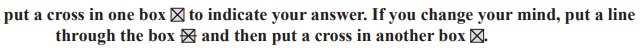
\includegraphics[width=15cm]{Year_6_Mixed_Tests/Xx.png}
\end{center}
 \\

 \begin{enumerate}
 
\item \quad \( 6532 \div 24 \)   \hspace{2cm} [2 marks] 
\vspace{90pt}
\hline
\vspace{5pt}

\item \quad \( 2436 \times 34 \) \hspace{2cm} [2 marks]
\vspace{90pt}
\hline
\vspace{5pt}

\item \quad \text{What is the value of the 6 in this number? }  \( 62345\)  \hspace{2cm} [2 marks]
\vspace{40pt}

\begin{center}
\begin{tabular}{c@{\hspace{3cm}}c@{\hspace{3cm}}c@{\hspace{3cm}}c}
  6 & 60 & 6000 & 60000 \\  
  
\includegraphics[width=1cm]{cross.png} & 
  
\includegraphics[width=1cm]{cross.png} & 
  
\includegraphics[width=1cm]{cross.png} & 
  
\includegraphics[width=1cm]{cross.png} \\
\end{tabular}
\end{center}
\hline
\vspace{10pt}

\item \quad \text{ What is 54678 rounded to the nearest hundred? } \hspace{2cm} [2 marks]
\vspace{20pt}

\begin{center}
\begin{tabular}{c@{\hspace{3cm}}c@{\hspace{3cm}}c@{\hspace{3cm}}c}
  50000 & 54700 & 54600 & 60000 \\
  
\includegraphics[width=1cm]{cross.png} & 
  
\includegraphics[width=1cm]{cross.png} & 
  
\includegraphics[width=1cm]{cross.png} & 
  
\includegraphics[width=1cm]{cross.png} \\
\end{tabular}
\end{center}
\hline
\vspace{10pt}

\item \quad \text{ What does 8 represent in 2564.678? } \hspace{2cm} [2 marks]
\vspace{20pt}

\begin{center}
\begin{tabular}{c@{\hspace{3cm}}c@{\hspace{3cm}}c@{\hspace{3cm}}c}
  Ones & Tenths & Hundredths & Thousandths \\
  
\includegraphics[width=1cm]{cross.png} & 
  
\includegraphics[width=1cm]{cross.png} & 
  
\includegraphics[width=1cm]{cross.png} & 
  
\includegraphics[width=1cm]{cross.png} \\
\end{tabular}
\end{center}
\hline
\vspace{10pt}

\item \text{ Write these numbers in order of size. Start with the smallest. } \hspace{2cm} [2 marks] \\
\begin{center}
5.06\hspace{2cm}5.006\hspace{2cm}56\% \hspace{2cm} \( \displaystyle \frac{5}{6}\) 
\vspace{30pt}

.......\hspace{2cm}.....\hspace{2cm}.....\hspace{2cm}.....\hspace{2cm}.....  \\
\end{center}
\hspace {2cm} Smallest

\vspace{10pt}

\item \quad \text{ Fill in A, B, C and D in the number line below. } \hspace{2cm} [2 marks]
\vspace{10pt}

 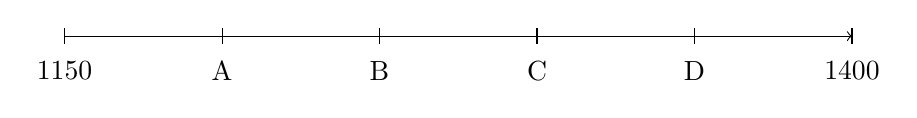
\begin{tikzpicture}
    % Draw the main line
    \draw[->] (0,0) -- (10,0);
    
    % Draw tick marks and labels
    \foreach \x/\label in {0/1150, 2/1200, 4/1250, 6/1300, 8/1350, 10/1400} {
        \draw (\x,-0.1) -- (\x,0.1);
        % Omit labels at positions 4 and 8 to leave them blank
        \ifnum\x=2 \else \ifnum\x=4 \else \ifnum\x=6 \else \ifnum\x=8 \else
            \node[below] at (\x,-0.2) {\label};
        \fi\fi\fi\fi
    }
    
    % Draw letters 'X' and 'Y' at positions 4 and 8
    \node[below] at (2,-0.2) {A};
    \node[below] at (4,-0.2) {B};
    \node[below] at (6,-0.2) {C};
    \node[below] at (8,-0.2) {D};
    
\end{tikzpicture}
\vspace{40pt}

\vspace{10pt}
\hline
\vspace{5pt}

% \item \quad \text{ Fill in A, B, C and D in the number line below. } 
% \vspace{40pt}

 % \begin{tikzpicture}
    % Draw the main line
   % \draw[->] (0,0) -- (10,0);
    
    % Draw tick marks and labels
   % \foreach \x/\label in {0/-400, 2/-200, 4/0, 6/200, 8/400, 10/600} {
       % \draw (\x,-0.1) -- (\x,0.1);
        % Omit labels at positions 4 and 8 to leave them blank
       % \ifnum\x=2 \else %\ifnum\x=4 \else 
      %  \ifnum\x=6 \else \ifnum\x=8 \else
     %       \node[below] at (\x,-0.2) {\label};
    %    \fi\fi\fi\fi
  %  }
    
    % Draw letters 'X' and 'Y' at positions 4 and 8
   % \node[below] at (2,-0.2) {A};
    %\node[below] at (4,-0.2) {B};
   % \node[below] at (6,-0.2) {C};
   % \node[below] at (8,-0.2) {D};
    
% \end{tikzpicture}

%\text{(9) Fill in X and Y in the number line below. } 
%\vspace{30pt}

 %\begin{tikzpicture}
    % Draw the main line
  %  \draw[->] (0,0) -- (10,0);
    
    % Draw tick marks and labels
   % \foreach \x/\label in {0/4000, 2/4200, 4/4400, 6/4600, 8/4800, 10/5000} {
    %    \draw (\x,-0.1) -- (\x,0.1);
        % Omit labels at positions 4 and 8 to leave them blank
     %   \ifnum\x=4 \else \ifnum\x=8 \else
      %      \node[below] at (\x,-0.2) {\label};
       % \fi\fi
    %}
    
    % Draw letters 'X' and 'Y' at positions 4 and 8
%   \node[below] at (4,-0.2) {A};
   % \node[below] at (8,-0.2) {B};
    
%\end{tikzpicture}

%\newpage

\item \quad \text{Write} \bm{\mathit{2876450}} \text{in words. } \hspace{2cm} [2 marks]
 %\text{(7) Write} \text{\textit{$\bm{38127}$}} \text{in words. } 
 \par
 \vspace{20pt}

\noindent \dotuline{\hspace{17cm}} \\
\par
\noindent \dotuline{\hspace{17cm}} \\
\vspace{10pt}
\hline
\vspace{10pt}

\item \quad \text{Write} \textit{\textbf{five million, six hundred and forty-nine thousand, eight hundred and }} \\
\textit{\textbf{twenty-three}} \text{in digits.} \hspace{2cm} [2 marks]

 
 \par
 \vspace{60pt}
 ..............................................

 \vspace{20pt}
 \hline
 \vspace{10pt}

\item (a) \quad \( 4^{2} + 18 \div (5-2 ) \) \hspace{2cm} [1 mark]
\vspace{80pt}
\hline
\vspace{10pt}

(b) \quad \( 8 + 2^{3} \div (7 - 3 ) \) \hspace {2cm} [1 mark]
\vspace{80pt}
\hline
\vspace{10pt}

\end{enumerate}
\end{document}